\chapter{Implementation details}
\label{ch:implementation_details}

This chapter aims to provide some insight into the technicalities in our development process, and to highlight the issues that we had to solve in order to get the final results. 

\section{\Maya Plugin}
\label{sec:maya_plugin}

We used rigs for \Maya that are provided for free by \cite{FaceWareRigsWeb}, the first thing to fix is to reset the paths for the textures in all the materials in the Hipershade window in \Maya.
The next step was to write plugin to load the weights from Matlab and set keyframes for each of them; to do this our plugin created a new \Maya command that could be easily executed. 
The work flow for writing the code was to first do the action in Maya manually if possible, see what MEL commands where executed, write them in the plugin and if possible rewrite them as pure C++ code instead of MEL commands.
Our code to complies with \Maya's undo command policy, which means using the \emph{DagModifier} class or including extra code to undo the actions.
Nevertheless, in the final stages of the implementation, it was faster to reload the scene that to undo the command.
The file format for the weights is one weight per line in frame order, as shown in Figure~\ref{fig:file_format}, where $N$ is the number of weights and $F$ is the number of frames.

\begin{figure}[htbp!]
\centering
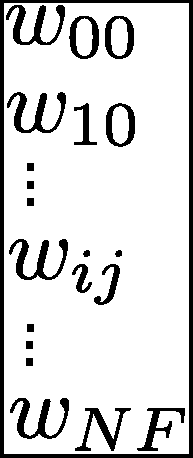
\includegraphics[width=0.1\textwidth]{img/file_format}
	\caption{File format for weights import and export.}
	\label{fig:file_format}
\end{figure}

After reading the weights  from the file, the connections between the blenshape object weights and its outputs have to be broken, this is done in order to be able to set the keyframes, otherwise the setKeyframe function would not work, an extract of the code is shown in Listing~\ref{lst:set_weights}.
An minor point to highlight in this section is that, the weights can be accessed using the following command, \textit{``shapesBS.weight[i]"}, however to break the connections the weight name in \Maya is needed.
To obtain a list with all the weights names the following command can be used, \textit{``listAttr -m shapesBS.w"}.
The weights will be listed in alphabetical order, yet the indices do not strictly follow the same order. 

\begin{lstlisting}[caption = Breaking the weights connections and setting keyframes., label = lst:set_weights, frame=single]

// Break connections.
for (unsigned int i = 0; i < (unsigned int)(numWeights); i++){
		cmd = "disconnectAttr shapesBS_";
		cmd = cmd + names[i];
		cmd = cmd + ".output shapesBS.";
		cmd = cmd + names[i];
		dgMod.commandToExecute(cmd);
}

// Set key frames
for (unsigned int j = 0; j < weights.at(i).size(); j++){
		cmd = "setAttr shapesBS.weight[";
		cmd = cmd + j;
		cmd = cmd + "] ";
		cmd = cmd + weights.at(i).at(j);
		dgMod.commandToExecute(cmd);
		
		cmd = "setKeyframe { \"shapesBS.w[";
		cmd = cmd + j;
		cmd = cmd + "]\" }";
		dgMod.commandToExecute(cmd);
	}
}
\end{lstlisting}

Once the weights were added, we noticed that the teeth and tongue of the Emily rig would not move.
Both meshes were actually regulated by the position of a control object in the scene, so the solution was to translate the object by a factor of the mean of all the weights involved in the mouth control, as shown in Listing~\ref{lst:teeth_tonge_control}.
The lower teeth and tongue would be left hanging mid air if the blendshapes that control the mouth opening were activated together; this problem was fixed by lowering the position of both meshes.

\begin{lstlisting}[caption = Teeth and tongue control based on relevant weights., label = lst:teeth_tonge_control, frame=single]

cmd = "setAttr con_jaw_c.translateY ";
cmd += -3.2 * (weights.at(i).at(58) + weights.at(i).at(55)) + 1;
dgMod.commandToExecute(cmd);
cmd = "setKeyframe  \"con_jaw_c.translateY\"";
dgMod.commandToExecute(cmd);
\end{lstlisting}

The next step was to include head rotation and translation back into the animation.
In order to achieve this, we saved the inverse rotation from the Procustes analisys that was performed on Section~\ref{sec:stabilising_head_movement}, into a file with the same format as shown in Figure~\ref{fig:file_format}.
We then read the data into \Maya and applied the transformation for each frame; for the translation we did a equivalent procedure with a translation file.
Note that Matlab matrices are column-wise while \Maya matrices are row-wise, so we read them taking into account this consideration.
The matrix multiplication order also plays in important role here, as shown in Equation~\ref{eq:rotation_translation_inv}, to achieve the correct result we need to undo the translation first and rotate the result.

\begin{equation}
\mathbf{x}_{new} = R\mathbf{x} + \mathbf{t} ~ \rightarrow  R^{-1}(\mathbf{x}_{new} - \mathbf{t}) = \mathbf{x},
\label{eq:rotation_translation_inv}
\end{equation}

where $\mathbf{x}$ is the original point, $\mathbf{x}_{new}$ is the transformed point, $R$ is the rotation matrix and $\mathbf{t}$ is a translation vector.
We implemented this transformation in \Maya using the ``xform -m" command, so we first apply the translation and then apply the rotation with an extra parameter ``-r" so that both matrices get multiplied in the desired order.

Having eye movement is quite important to achieve realism in the animation, for this purpose we tracked the pupils' world positions in the input frame sequence.
These positions were saved into separate files for each eye using the format shown in Figure~\ref{fig:file_format}.
The positions were loaded into \Maya and the eye control object was translated using the offsets with respect to the first frame, which was assumed to be looking straight.
With this first approach each eye can move independently which leads to unsatisfactory results, an initial solution to this problem was to move both eyes using the mean offset for each frame.
Nevertheless, this would introduce considerable error when one of the eyes winks, as the tracking becomes completely unreliable for the winking eye which in turn drags the other eye.
Our solution involves interpolating between the two offsets using variable factors.
The idea is to have both eyes moving together, start ignoring the offset for an eye if it goes off, while sustaining smooth movements.
The final offset $d_f$ will be computed as $d_f = \alpha d_l + \beta d_r$, where $\alpha$ and $\beta$ are the interpolation factors, $d_l$ and $d_r$ are the offsets for the left and right eye, respectively.
Figure~\ref{fig:eyes_interpolation} shows the $\alpha_x$ values along the $x$ direction, where $t$ is the change threshold and $l$ is the maximum offset limit.
Initially $\alpha_x$ is $0.5$, however if the offset goes beyond a threshold $t$, $\alpha$ will decrease linearly until it reaches the limit $l$.
The same criteria will be applied in the $y$ direction, and the value for that eye will be $\alpha = \min \left\lbrace \alpha_x, \alpha_y \right\rbrace$.
The $\beta$ factor will be computed as $\beta = 1 - \alpha$, however, if the right eye is the one surpassing the threshold $t$, then the whole process will be reversed. 
Additionally, if both eyes surpass the threshold $t$, $\alpha$ and $\beta$ will be $0.5$, this will allow the eyes to move together beyond the threshold if needed.

\begin{figure}[htbp!]
\centering
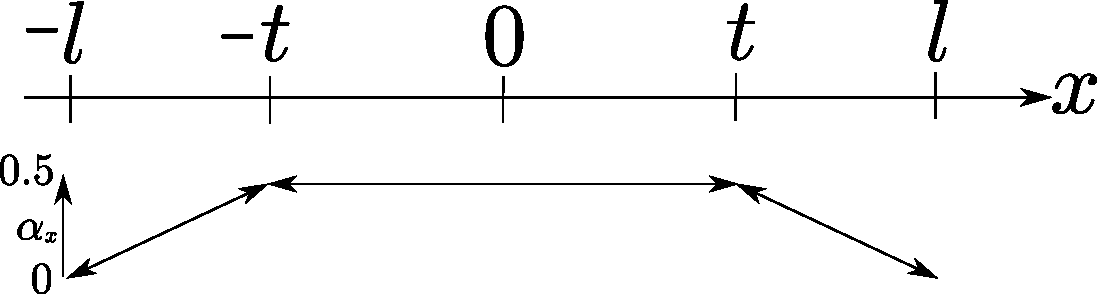
\includegraphics[width=0.8\textwidth]{img/eyes_interpolation}
	\caption{Offset interpolation for eye movements in \Maya.}
	\label{fig:eyes_interpolation}
\end{figure}

Incorporating blinks was another important step towards attaining a more realistic animation.
Since the eyelids were not tracked in the recording session, the only option was to manually set the blinking times in \Maya.
To faithfully reproduce the blinking in the data the following information was manually added:
\begin{itemize}
\item Frame number marking when the eye:
	\begin{itemize}
	\item started closing;
	\item closed completely;
	\item started opening again;
	\item was fully open again;
	\end{itemize}
\item The blink magnitude (eyes fully close, squinting, etc);
\item The blink type (both eyes closed, only one eye).
\end{itemize}

As mentioned in Section~\ref{sec:estimation_w_actor_domain}, there is a mismatch between Emily's neutral face and the actor's neutral face.
In order to disguise this discrepancy as much as possible, a fixed constant was added to the blenshape weights controlling the smile, we found that the best value for this constant was $0.35$.

%-----------------------------------------------------------------------------------------

\section{Skin Rendering}

Initially for all the Image Analogies work we used an implementation based on~\cite{ImAnSingleThreadWeb}.
This library was quite slow and it would not give results as good as the ones shown in the original paper.
We then moved to a parallel CUDA implementation~\cite{ImAnCudaWeb}; with this code the problem was inconsisten results depending on the number of threads and erroneous pixel values, as shown in Figure~\ref{fig:cuda_error}.
The original code for Image Analogies has not been maintained since 2001, a patched version of the library, along with instruction on how to compile and run the code are provided alongside this report.

\begin{figure}[htbp!]
\centering
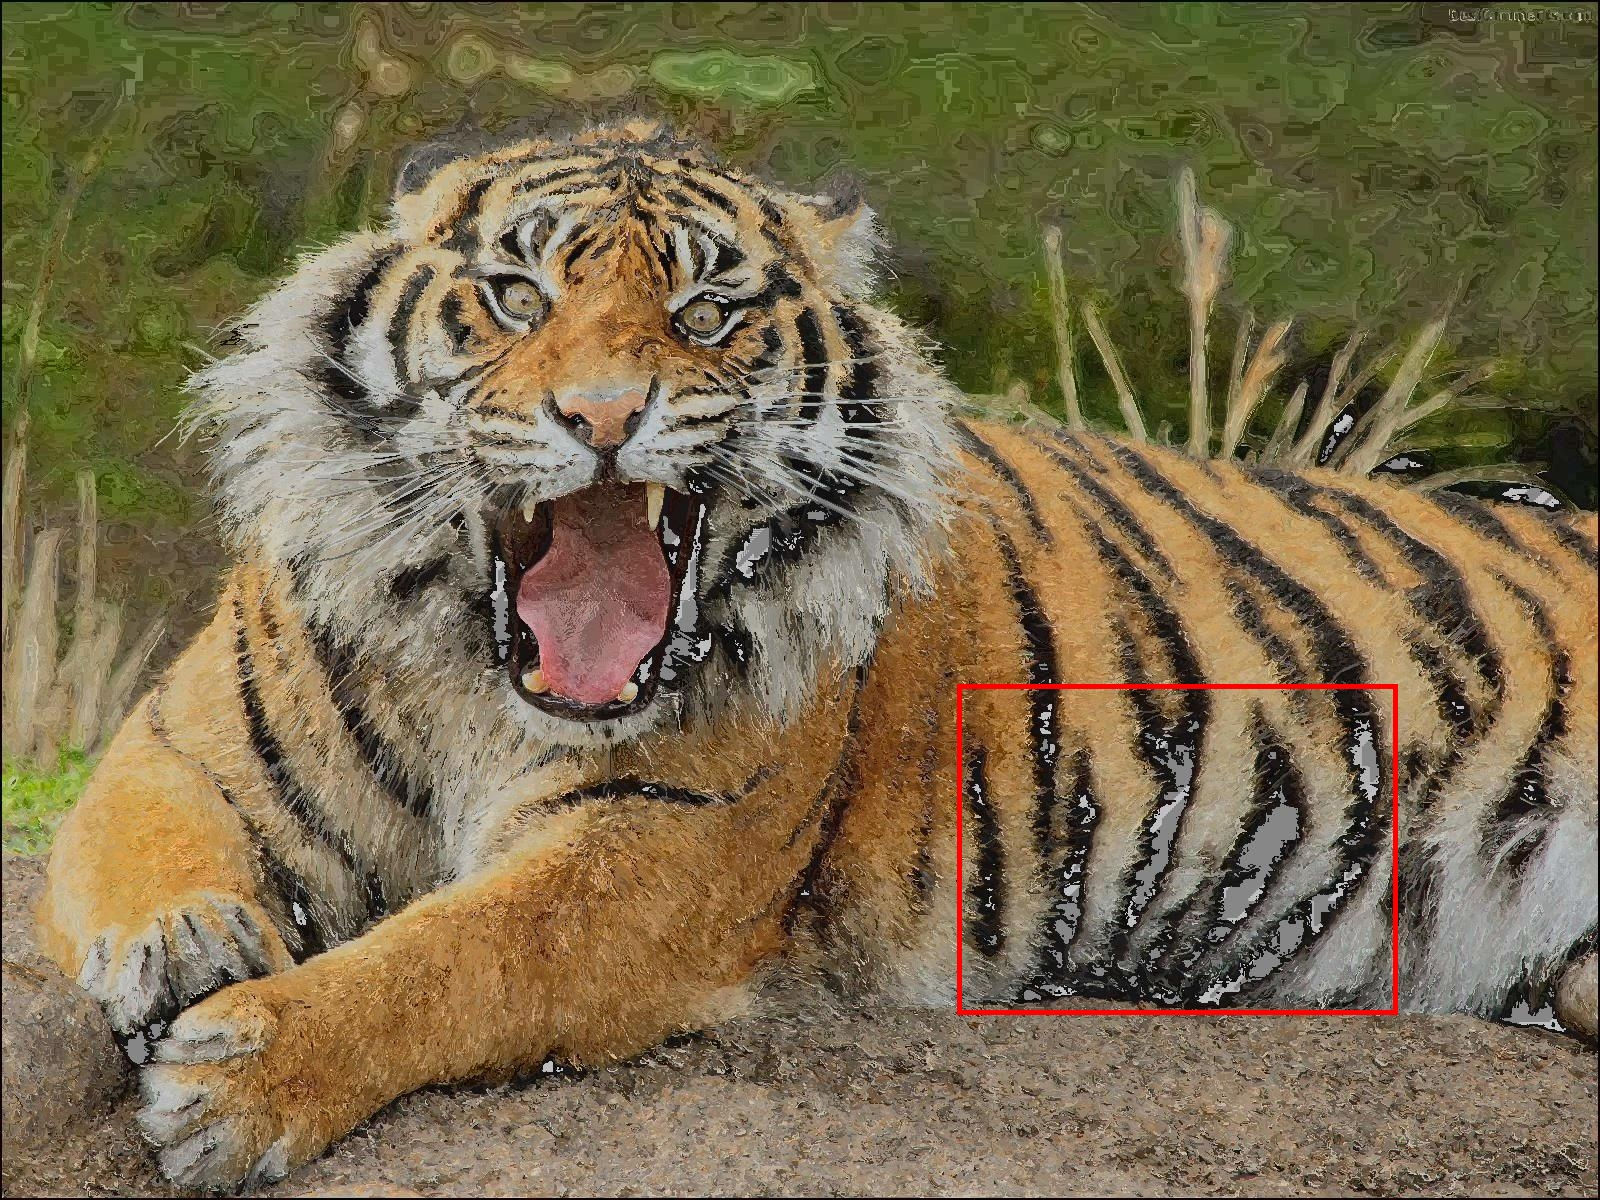
\includegraphics[width=0.5\textwidth]{img/cuda_error}
	\caption{Result for CUDA image analogy implementation, erroneous values highlighted in the red square, image taken from~\cite{ImAnCudaWeb}.}
	\label{fig:cuda_error}
\end{figure}

There are two important problems when using Image Analogies filter for adding detail to textures.
The first one arises due to the difference in colour distributions between the inputs.
For our data, this mismatch between $\left\lbrace A, A' \right\rbrace$ and $B$, was caused by divergent lighting conditions in the capture studio.
Since we have the prior knowledge that the images should represent the same areas, we applied colour correction techniques to match the images.
The second issue derives from the local texture patch growth that the algorithm uses to replicate coherent patches in the input images.
If the kernel sizes do not match the features that we want to preserve in the example images, unconnected patches will be produced.
Moreover, this problem will be exacerbated with the face segmentation approach that was presented in Section~\ref{sec:metho_skin_rendering}.
In Figure~\ref{fig:skin_patch_error}, the top half of the image shows an example of kernel size error, and the seam between the two zones is quite evident due to the patch segmentation.

\begin{figure}[htbp!]
\centering
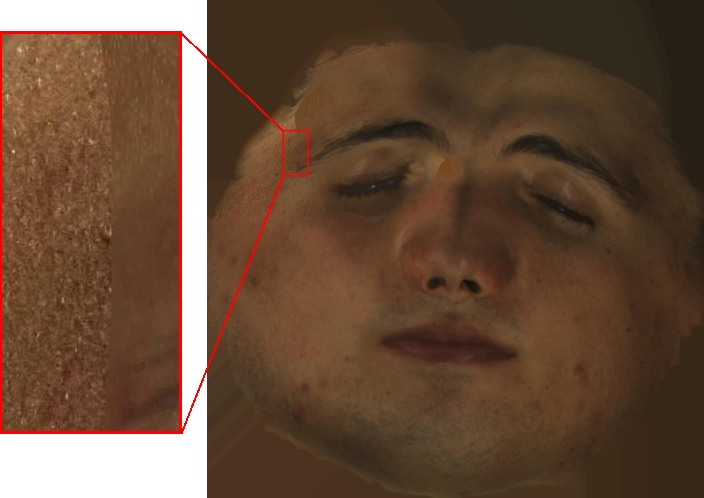
\includegraphics[width=0.6\textwidth]{img/skin_patch_error}
	\caption{Erroneously generated skin texture.}
	\label{fig:skin_patch_error}
\end{figure}


\section{Matlab}

